\documentclass[tikz,border=0pt]{standalone}
\usepackage[T1]{fontenc}
\usepackage{tgheros}
\usepackage{graphicx}
\usepackage{newtxmath}
\usetikzlibrary{arrows.meta}
\renewcommand{\familydefault}{\sfdefault}

\definecolor{ink}{HTML}{172C3D}
\definecolor{muted}{HTML}{4D626F}
\definecolor{bluePanel}{HTML}{EDF3F8}
\definecolor{blueEdge}{HTML}{A5B8C9}
\definecolor{teal}{HTML}{147D75}
\definecolor{tealPanel}{HTML}{EAF6F3}
\definecolor{tealEdge}{HTML}{A6CBC4}
\definecolor{amber}{HTML}{9B5C21}
\definecolor{amberPanel}{HTML}{FFF4E7}
\definecolor{amberEdge}{HTML}{DBC1A2}
% Legend colours match the Figures4Papers-inspired Matplotlib capital panel.
\definecolor{assetA}{HTML}{0F4D92}
\definecolor{assetB}{HTML}{3775BA}
\definecolor{assetC}{HTML}{A6C5E6}
\definecolor{cash}{HTML}{CFCECE}

\begin{document}
\begin{tikzpicture}[
  x=1mm,y=1mm,text=ink,font=\sffamily\fontsize{8.1}{9.5}\selectfont,
  panel/.style={draw,rounded corners=2.6pt,line width=.48pt},
  card/.style={fill=white,draw,rounded corners=1.6pt,line width=.42pt},
  heading/.style={anchor=west,inner sep=0pt,font=\sffamily\bfseries\fontsize{9.6}{11}\selectfont},
  label/.style={anchor=west,inner sep=0pt,font=\sffamily\bfseries\fontsize{7.8}{9}\selectfont},
  copy/.style={anchor=west,inner sep=0pt,align=left},
  note/.style={anchor=west,inner sep=0pt,align=left,text=muted,
    font=\sffamily\fontsize{7.35}{8.5}\selectfont},
  arrow/.style={-{Stealth[length=3.9pt,width=3.4pt]},line width=.75pt}
]
\path[use as bounding box] (-4.4,0) rectangle (122,125);

% Market observations available at the decision cutoff.
\draw[panel,draw=blueEdge,fill=bluePanel] (.25,101.25) rectangle (121.75,124.75);
\fill[blueEdge!33,rounded corners=1.7pt] (.7,116.25) rectangle (121.3,124.3);
\node[heading] at (3.6,120.25) {Market observations at close $t$};
\node[note,anchor=east] at (118.6,120.25) {Illustrative stock example};
\draw[blueEdge,line width=.43pt] (39.4,103.7) -- (39.4,114.2)
  (82.1,103.7) -- (82.1,114.2);

% Price tape, document and clock pictograms identify the input types.
\draw[amber!73,line width=.54pt] (4.4,105.3) -- (4.4,113.3)
  (4.4,105.3) -- (15,105.3);
\draw[amber,line width=.9pt,line cap=round,line join=round]
  (5.3,107) -- (7.1,109) -- (9.1,108.1) -- (11,110.8) -- (12.4,110.2) -- (14.7,112.8);
\node[label] at (16.3,110.65) {Adjusted closes};
\node[note] at (16.3,106.75) {Price history};

\draw[teal,fill=white,line width=.61pt,line join=round] (43,104.9)
  -- (43,113.4) -- (48.4,113.4) -- (50.4,111.4) -- (50.4,104.9) -- cycle;
\draw[teal,line width=.52pt] (48.4,113.4) -- (48.4,111.4) -- (50.4,111.4)
  (44.5,110.5) -- (47.4,110.5)
  (44.5,108.9) -- (48.9,108.9)
  (44.5,107.3) -- (48.2,107.3);
\node[label] at (53,110.65) {Company news};
\node[note] at (53,106.75) {Dated articles};

\draw[fill=white,draw=ink,line width=.59pt] (89.1,109.2) circle[radius=4.0mm];
\draw[draw=ink,line width=.65pt,line cap=round] (89.1,111.55)
  -- (89.1,109.2) -- (91,108.3);
\node[label] at (95.5,110.65) {Decision cutoff};
\node[note] at (95.5,106.75) {Daily close $t$};

\draw[arrow,teal,rounded corners=1.2pt] (59,100.9) -- (59,97.9)
  -- (17,97.9) -- (17,95.3);
\draw[arrow,amber,rounded corners=1.3pt] (-.1,109.2) -- (-3.5,109.2)
  -- (-3.5,22.1) -- (-.15,22.1);

% News extraction and relative allocation.
\begin{scope}[yshift=8mm]
\draw[panel,draw=tealEdge,fill=tealPanel] (.25,44.5) rectangle (121.75,86.75);
\fill[teal!13,rounded corners=1.7pt] (.7,77.9) rectangle (121.3,86.3);
\node[heading] at (3.6,82.35) {(a)\enspace From financial news to relative weights};


\node[label] at (3.7,75.5) {Dated headlines};
\node[label] at (34.7,75.5) {LLM event records};
\draw[teal,fill=white,line width=.49pt,rounded corners=.45pt]
  (64.35,74.1) rectangle (67.1,76.85);
\draw[teal,line width=.44pt] (65.1,76.85) -- (65.1,77.35)
  (66.35,76.85) -- (66.35,77.35)
  (65.1,74.1) -- (65.1,73.6)
  (66.35,74.1) -- (66.35,73.6)
  (64.35,74.85) -- (63.8,74.85)
  (64.35,76.1) -- (63.8,76.1)
  (67.1,74.85) -- (67.65,74.85)
  (67.1,76.1) -- (67.65,76.1);
\fill[teal!55] (65.1,74.85) rectangle (66.35,76.1);
\node[label] at (78.8,75.5) {Scores and rank-tilted shares};

\draw[card,draw=tealEdge] (3.6,60.8) rectangle (29.7,72.2);
\draw[card,draw=tealEdge] (3.6,46.9) rectangle (29.7,58.3);
\draw[teal,line width=1.15pt] (3.85,62.2) -- (3.85,70.8);
\draw[cash,line width=1.15pt] (3.85,48.3) -- (3.85,56.9);
\node[copy] at (5.6,66.5) {A raises FY\\[-.4pt] guidance to \$5bn};
\node[copy] at (5.6,52.6) {B mentioned in\\[-.4pt] a sector roundup};

\draw[card,draw=tealEdge] (34.6,60.8) rectangle (73.8,72.2);
\draw[card,draw=tealEdge] (34.6,46.9) rectangle (73.8,58.3);
\node[copy] at (36.4,68.8) {\textbf{A}~~Main subject};
\node[note] at (36.4,64) {Figures, new guidance};
\draw[fill=tealPanel,draw=tealEdge,rounded corners=1pt,line width=.38pt]
  (64.6,62.4) rectangle (72.2,70.6);
\node[note,anchor=center,font=\sffamily\fontsize{6.5}{7.5}\selectfont]
  at (68.4,68.5) {Impact};
\node[text=teal,font=\sffamily\bfseries\fontsize{8}{9}\selectfont,inner sep=0pt]
  at (68.4,64.95) {$+2$};
\node[copy] at (36.4,54.9) {\textbf{B}~~Mention only, no figures};
\node[note] at (36.4,50) {Excluded by the gate};

\draw[arrow,teal] (30.2,66.5) -- (34,66.5);
\draw[arrow,muted] (30.2,52.6) -- (34,52.6);
\draw[arrow,teal] (74.3,66.5) -- (78.1,66.5);

% The mini-chart makes the ordering visible independently of the signed score labels.
\draw[card,draw=tealEdge] (78.8,46.9) rectangle (118.6,72.2);
\node[note] at (80.5,69.4) {Asset};
\node[note,anchor=center] at (97.8,69.4) {EMA score $s_{i,t}$};
\node[note,anchor=center] at (114.4,69.4) {$q_{i,t}$};
\draw[tealEdge,line width=.4pt] (80.3,66.9) -- (117.1,66.9);
\draw[muted!48,line width=.4pt] (92.7,50.3) -- (92.7,66.3);
\foreach \asset/\pos/\extent/\value/\share in {
  A/64/8.2/{+0.30}/{1/2}, B/58.5/2.187/{+0.08}/{1/3}, C/53/-4.373/{-0.16}/{1/6}} {
  \node[copy] at (81,\pos) {\textbf{\asset}};
  \fill[teal!77] (92.7,{\pos-.73}) rectangle ({92.7+\extent},{\pos+.73});
  \node[anchor=east,inner sep=0pt] at (109,\pos) {$\value$};
  \node[inner sep=0pt] at (114.4,\pos) {$\share$};
}
\node[note] at (80.5,49.2) {Earlier scores can persist};

\end{scope}

% The current rank tilt can reach this computation only after another price return.
\draw[arrow,teal,densely dashed,rounded corners=1.4pt]
  (97.3,52.1) -- (97.3,45.6) -- (40.35,45.6) -- (40.35,40.95);
\node[note,anchor=center] at (68.65,48.25) {Tilt enters risk after a later return};

% Volatility estimates use an illustrative 20-return series with ~25% annualised volatility.
\draw[panel,draw=amberEdge,fill=amberPanel] (.25,.25) rectangle (73.95,40.55);
\fill[amber!15,rounded corners=1.7pt] (.7,32.4) rectangle (73.5,40.1);
\node[heading] at (3.6,36.15) {(b)\enspace From realised volatility to budget};
\node[note] at (3.7,30.6) {Returns weighted by previous tilts};
\node[note,anchor=center] at (24.7,3.8) {Trailing 20 panel dates};
\draw[card,draw=amberEdge] (3.6,7) rectangle (45.85,27.9);
\node[anchor=south west,inner sep=0pt] at (4.4,7.65)
  {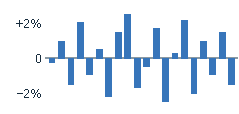
\includegraphics{voltilt_figure_panels/returns_overview.pdf}};

\draw[card,draw=amberEdge] (50.2,7) rectangle (70.55,27.9);
\node[note,anchor=center] at (60.375,24.6) {Annualised vol.};
\node[inner sep=0pt] at (60.375,20.6) {$\hat{\sigma}_t=25\%$};
\draw[amberEdge,line width=.45pt] (52.1,17.7) -- (68.65,17.7);
\node[note,anchor=center] at (60.375,14.4) {20\% target};
\node[inner sep=0pt,font=\fontsize{8.6}{10}\selectfont]
  at (60.375,10.7) {$\lambda_t=0.80$};
\draw[arrow,amber] (46.25,17.5) -- (49.75,17.5);

% Risky weights in the bar and ledger are shares of total capital.
\draw[panel,draw=blueEdge,fill=bluePanel] (78.6,.25) rectangle (121.75,40.55);
\fill[blueEdge!33,rounded corners=1.7pt] (79.05,32.4) rectangle (121.3,40.1);
\node[heading] at (82.1,36.15) {(c)\enspace Capital allocation};
\node[inner sep=0pt,font=\fontsize{10}{12}\selectfont] at (100.2,28.1)
  {$a_{i,t}=\lambda_t q_{i,t}$};

\node[anchor=south west,inner sep=0pt] at (82.1,19)
  {
\includegraphics{voltilt_figure_panels/capital_overview.pdf}};
\foreach \x/\y/\tone/\asset/\weight in {
  82.1/13.4/assetA/A/40,
  82.1/7.4/assetB/B/26.7,
  101.4/13.4/assetC/C/13.3,
  101.4/7.4/cash/Cash/20} {
  \fill[\tone] (\x,{\y-1.05}) rectangle ++(2.15,2.1);
  \node[copy] at ({\x+3.25},\y) {\asset\ \weight\%};
}
\draw[arrow,teal] (114.4,52.1) -- (114.4,41);
\draw[arrow,amber] (74.35,17.5) -- (78.15,17.5);
\end{tikzpicture}
\end{document}
